\begin{enumerate}
	\item Длины базисных векторов $\vec e_1, \vec e_2, \vec e_3$ равны $\sqrt 3, 3$ и $2$ соответственно. Углы между ними равны $\angle(\vec e_1, \vec e_2) = 90^\circ, \angle(\vec e_2, \vec e_3) = 60^\circ, \angle(\vec e_1, \vec e_3) = 30^\circ$. Вычислите высоты параллелограмма, построенного на векторах, имеющих в этом базисе координаты $\vec a (-3, 1, 0)^T$ и $\vec b (1, 0, -2)^T$.

	 	  \item Выведите формулу Лагранжа двойного векторного произведения.
	 	
	 \item Вычислить $[\vec a,[\vec b, \vec c]]$, если 
	$$\vec a = \begin{pmatrix}
	    	1 \\ 2 \\ 3
	    \end{pmatrix},\quad
	   \vec b = \begin{pmatrix}
	    	3 \\ 2 \\ 1	    
	    \end{pmatrix},\quad
	    \vec c = \begin{pmatrix}
	    	1 \\ 1 \\ 1  
	    \end{pmatrix} $$
	    Базис считать ортонормированным. 
	    

	  \item Сформулируйте и выведите критерий коллинеарности векторов в пространстве (вы можете пользоваться следующим пока не доказанным свойством: если векторы $\vec e_1, \vec e_2, \vec e_3$ некомпланарны, то и их попарные векторные произведения тоже некомпланарны).
	
	  
	  \item Используя свойства скалярного произведения, докажите, что у любого параллелограмма сумма квадратов длин диагоналей равна сумме квадратов длин всех его сторон.
	  
	  \item Дан треугольник $\triangle ABC$. Найдите отношение площади $S$ треугольника, составленного из его медиан $AA_1, BB_1, CC_1$, к площади $S_0$ исходного треугольника $ABC$.
	  \begin{figure*}[ht]
	  	\centering
	  	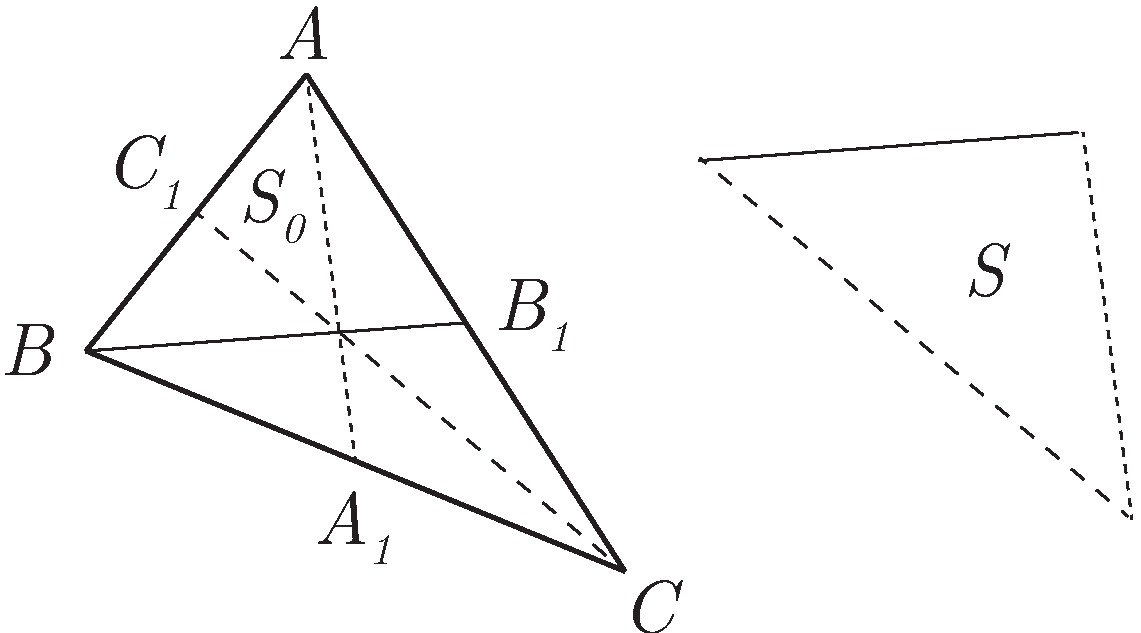
\includegraphics[width=0.4\textwidth]{triangle}
	  \end{figure*}
	  
	  \item Объяснить при заданных $\vec a$ и $p$ геометрический смысл всех решений уравнения $(\vec x, \vec a) = p$
	    \begin{tasks}(1)
		        \task на плоскости
		        \task в пространстве 
	    \end{tasks}
	  \end{enumerate}